\documentclass[twoside]{article}

\usepackage[accepted]{aistats2021}

% to compile a preprint version, e.g., for submission to arXiv, add add the
% [preprint] option:
    %  \usepackage[preprint]{neurips_2020}

% to compile a camera-ready version, add the [final] option, e.g.:
%     \usepackage[final]{neurips_2020}

% to avoid loading the natbib package, add option nonatbib:
    %  \usepackage[nonatbib]{neurips_2020}

\usepackage[utf8]{inputenc} % allow utf-8 input
\usepackage[T1]{fontenc}    % use 8-bit T1 fonts
\special{papersize = 8.5in, 11in}
\setlength{\pdfpageheight}{11in}
\setlength{\pdfpagewidth}{8.5in}
\usepackage[colorlinks]{hyperref}       % hyperlinks
\hypersetup{
    colorlinks = true,
    linkcolor = blue,
    anchorcolor = blue,
    citecolor = blue,
    filecolor = blue,
    urlcolor = blue
}

\usepackage{url}            % simple URL typesetting
\usepackage{booktabs}       % professional-quality tables
\usepackage{amsfonts}       % blackboard math symbols
\usepackage{amsmath}
\usepackage{nicefrac}       % compact symbols for 1/2, etc.
\usepackage{xcolor}
\usepackage{algorithm}
\usepackage[noend]{algpseudocode}
\newcommand{\sfunction}[1]{\textsf{\textsc{#1}}}
\algrenewcommand\algorithmicforall{\textbf{foreach}}
\usepackage{textcomp}
\usepackage{subcaption,graphicx}
\usepackage[font=footnotesize,labelfont=bf]{caption}

\usepackage{array,multirow}

\usepackage{accents}

\usepackage{ntheorem}
\usepackage[nomessages]{fp}% http://ctan.org/pkg/fp

% Math text commands
\newcommand{\mathcal}{\mathcal}
\newcommand{\mathbf}{\boldsymbol}
\newcommand{\mathbb}{\mathbb}

% Math new operators
\DeclareMathOperator*{\argmax}{arg\,max}
\DeclareMathOperator*{\trace}{trace}
\DeclareMathOperator*{\diag}{diag}
\DeclareMathOperator*{\argmin}{arg\,min}
\DeclareMathOperator*{\tr}{tr}
\DeclareMathOperator{\dt}{\, \mathrm{d}\mathit{t}}
\newcommand{\abs}[1]{\left\lvert #1 \right\rvert}
\newcommand\independent{\protect\mathpalette{\protect\independenT}{\perp}}

\usepackage{xstring}

% Math braces
\newcommand{\brac}[1]{\left({#1}\right)}
\newcommand{\sbrac}[1]{\left[{#1}\right]}
\newcommand{\cbrac}[1]{\left\{{#1}\right\}}

\newcommand{\bestresult}[2]{\FPeval{\m}{round(#1, 2)}\FPeval{\s}{round(#2, 2)} \StrGobbleLeft{\s}{1}[\s]${\scriptstyle \mathbf{\m_{{\pm \s}}}}$}
\newcommand{\result}[2]{\FPeval{\m}{round(#1, 2)}\FPeval{\s}{round(#2, 2)} \StrGobbleLeft{\s}{1}[\s]${\scriptstyle \m_{\scriptstyle \pm \s}}$}

\usepackage{mathtools}
\DeclarePairedDelimiter{\ceil}{\lceil}{\rceil}
\DeclarePairedDelimiter{\floor}{\lfloor}{\rfloor}

% Theorems:
\usepackage{amsthm}
\newtheorem{proposition}{Proposition}[section]


% Comments commands:
\newcommand{\gilles}[1]{\textcolor{red}{[GL: #1]}}
\newcommand{\antoine}[1]{\textcolor{orange}{[AW: #1]}}
\newcommand{\textbf}[1]{\textbf{#1}}
\newcommand{\figref}[1]{Fig.~\ref{#1}}
\newcommand{\Cref}[1]{Table~\ref{#1}}

%\usepackage{tikz}
% \usepackage{includetikz}
% \usetikzlibrary{positioning,fit,calc,decorations.pathreplacing,arrows,backgrounds}
\usepackage{relsize}
\usepackage{tikz}
\usetikzlibrary{positioning,fit,calc,decorations.pathreplacing,arrows,backgrounds,shapes}
\usetikzlibrary{decorations.pathreplacing,angles,quotes}

\usetikzlibrary{automata,arrows}


%%% Algorithm commands %%%%
\newcommand{\pushline}{\Indp}% Indent
\newcommand{\popline}{\Indm\dosemic}% Undent
\newcommand{\nonl}{\renewcommand{\nl}{\let\nl\oldnl}}% Remove line number for one line


% The \author macro works with any number of authors. There are two commands
% used to separate the names and addresses of multiple authors: \And and \AND.
%
% Using \And between authors leaves it to LaTeX to determine where to break the
% lines. Using \AND forces a line break at that point. So, if LaTeX puts 3 of 4
% authors names on the first line, and the last on the second line, try using
% \AND instead of \And before the third author name.

% %\author{
%   Antoine Wehenkel \\
%   University of Liège \\
%   % Address \\
%   \texttt{antoine.wehenkel@uliege.be} \\
%   \And
%   Gilles Louppe \\
%   University of Liège \\
%   % Address \\
%   \texttt{g.louppe@uliege.be} \\
%   % \And
%   % Coauthor \\
%   % Affiliation \\
%   % Address \\
%   % \texttt{email} \\
%   % \And
%   % Coauthor \\
%   % Affiliation \\
%   % Address \\
%   % \texttt{email} \\
% }
\usepackage[]{natbib}
\bibliographystyle{plainnat}

\begin{document}

\twocolumn[
\aistatstitle{Graphical Normalizing Flows}

\aistatsauthor{ Antoine Wehenkel \And Gilles Louppe }

\aistatsaddress{ ULiège \And ULiège} ]

\begin{abstract}
Normalizing flows model complex probability distributions by combining a base distribution with a series of bijective neural networks. State-of-the-art architectures rely on coupling and autoregressive transformations to lift up invertible functions from scalars to vectors.
In this work, we revisit these transformations as probabilistic graphical models, showing they reduce to Bayesian networks with a pre-defined topology and a learnable density at each node.
From this new perspective, we propose the graphical normalizing flow, a new invertible transformation with either a prescribed or a learnable graphical structure.
This model provides a promising way to inject domain knowledge into normalizing flows while preserving both the interpretability of Bayesian networks and the representation capacity of normalizing flows. We show that graphical conditioners discover relevant graph structure when we cannot hypothesize it. In addition, we analyze the effect of $\ell_1$-penalization on the recovered structure and on the quality of the resulting density estimation. Finally, we show that graphical conditioners lead to competitive white box density estimators.
Our implementation is available at \url{https://github.com/AWehenkel/DAG-NF}.
\end{abstract}

\section{Introduction}
Normalizing flows~\citep[NFs, ][]{NF, tabak2010density, tabak2013family, rippel2013high} have proven to be an effective way to model complex data distributions with neural networks. These models map data points to latent variables through an invertible function while keeping track of the change of density caused by the transformation. In contrast to variational auto-encoders (VAEs) and generative adversarial networks (GANs), NFs provide access to the exact likelihood of the model's parameters, hence offering a sound and direct way to optimize the network parameters. Normalizing flows have proven to be of practical interest as demonstrated by \citet{parallel_wavenet, kim2018flowavenet} and \citet{ prenger2019waveglow} for speech synthesis, by \citet{NF, kingma2016improved} and \citet{berg2018sylvester} for variational inference or by \citet{SNL} and \citet{greenberg2019automatic} for simulation-based inference. Yet, their usage as a base component of the machine learning toolbox is still limited in comparison to GANs or VAEs. Recent efforts have been made by \citet{flows-review} and \citet{flow_review_2} to define the fundamental principles of flow design and by \citet{neural-spline-flows} to provide coding tools for modular implementations. We argue that normalizing flows would gain in popularity by offering stronger inductive bias as well as more interpretability. %Moreover, some fundamental properties of NFs are still to be understood and we believe that to do so could lead to long-term improvements in the field.% and by being more intuitive to build. %\cite{flows-tori} makes a similar observation to motivate their flow on non-euclidean space.
%\antoine{And improvement if better understood}

Sometimes forgotten in favor of more data oriented methods, probabilistic graphical models (PGMs) have been popular for modeling complex data distributions while being relatively simple to build and read \citep{PGM-book, johnson2016composing}. Among PGMs, Bayesian networks~\citep[BNs, ][]{Pearl-BN} offer an appealing balance between modeling capacity and simplicity. Most notably, these models have been at the basis of expert systems before the big data era (e.g. \citep{BN-app-1, BN-app-2, BN-app-3}) and were commonly used to merge qualitative expert knowledge and quantitative information together. On the one hand, experts stated independence assumptions that should be encoded by the structure of the network. On the other hand, data were used to estimate the parameters of the conditional probabilities/densities encoding the quantitative aspects of the data distribution. %B-net are closely related to the field of causality by being a super-set of causal graphical models.
These models have progressively received less attention from the machine learning community in favor of other methods that scale better with the dimensionality of the data. %Moreover, practical applications for continuous data stands on a strong hypothesis on the class of distributions combined with linear dependence relationships that limits the modeling capacities.
% most of the results for continuous data have been found with Gaussian assumption and linear relationships combined with Gaussian distributions \citep{geiger1994learning} or by discretization \citep{friedman1998bayesian}, they do not offer any standard way to model continuous data.
%\antoine{Causal Models?}

% Driven by the ambition to bring intuition into normalizing flows and the already proven relevance of BNs for combining qualitative and quantitative reasoning, we review normalizing flows under the lens of Bayesian networks. We show that autoregressive and coupling transformations can be seen as BNs with a predefined topology. Based on the gained insights, we propose a new building block that allows normalizing flows to be directly related to BNs without any constraint on the topology, laying additional space for inductive bias into normalizing flows.
Driven by the objective of integrating intuition into normalizing flows and the proven relevance of BNs for combining qualitative and quantitative reasoning, we summarize our contributions as follows:
\textbf{(i)} From the insight that coupling and autoregressive transformations can be reduced to Bayesian networks with a fixed topology, we introduce the more general graphical conditioner for normalizing flows, featuring either a prescribed or a learnable BN topology; \textbf{(ii)} We show that using a correct prescribed topology leads to improvements in the modeled density compared to autoregressive methods. When the topology is not known we observe that, with the right amount of $\ell_1$-penalization, graphical conditioners discover relevant relationships; \textbf{(iii)} In addition, we show that graphical normalizing flows perform well in a large variety of density estimation tasks compared to classical black-box flow architectures.
% \begin{itemize}
%     %\item We provide a new vision of coupling and autoregressive transformations as Bayesian Networks.
%     %\item Thanks to this new tool, we provide proofs and insights on some of the fundamental properties of Normalizing Flows.
%     \item From the insight that coupling and autoregressive transformations can be reduced to Bayesian networks with a fixed topology, we introduce the more general graphical conditioner for normalizing flows, featuring either a prescribed or a learnable BN topology.
%     \item We show that using a correct prescribed topology leads to improvements in the modeled density compared to autoregressive methods. When the topology is not known we observe that, with the right amount of $\ell_1$-penalization, graphical conditioners discover relevant relationships.
%     \item In addition, we show that graphical normalizing flows perform well in a large variety of density estimation tasks compared to classical black-box flow architectures.
%     %They are not only competitive as a black-box normalizing flow, but also provide an operational way to introduce domain knowledge into neural network based density estimation.
% \end{itemize}
%%%%%%%%%%%%%%%%%%%%%%% Section 2
\section{Background}

\paragraph{Bayesian networks}
A Bayesian network is a directed acyclic graph (DAG) that represents independence assumptions between the components of a random vector. Formally, let $\mathbf{x} = \left[x_1, \hdots, x_d\right]^T \in \mathbb{R}^d$ be a random vector distributed under $p_{\mathbf{x}}$. A BN associated to $\mathbf{x}$ is a directed acyclic graph made of $d$ vertices representing the components $x_i$ of $\mathbf{x}$. In this kind of network, the absence of edges models conditional independence between groups of components through the concept of d-separation~\citep{d-separation}. A BN is a valid representation of a random vector $\mathbf{x}$ iff its density can be factorized as
\begin{align}
    p_{\mathbf{x}}(\mathbf{x}) = \prod^d_{i=1}p(x_i|\mathcal{P}_i),\label{eq:BN-fact}
\end{align}
where  $\mathcal{P}_i = \{j: A_{i,j} = 1 \}$ denotes the set of parents of the vertex $i$ and $A \in \{0, 1\}^{d\times d}$ is the adjacency matrix of the BN. As an example, \figref{fig:mono-step-flows-a} is a valid BN for any distribution over $\mathbf{x}$ because it does not state any independence and leads to a factorization that corresponds to the chain rule. However, in practice we seek for a sparse and valid BN which models most of the independence between the components of $\mathbf{x}$, leading to an efficient factorization of the modeled probability distribution. It is worth noting that making hypotheses on the graph structure is equivalent to assuming certain conditional independence between some of the vector's components.
%In our experiments the parameters of the neural networks encoding for the monotonic transformations $g^i$ are shared, they take as input a one hot encoding vector that represents the index $i$.

%BNs and probabilistic graphical models in general are popular because they compactly describe probability distributions over random vectors. First, a sparse network will lead to an efficient factorization of the probability distribution. Indeed, the more sparse the BN is, the smaller the average size of the input space of the conditioning factors is. Second, the d-separation algorithm is an efficient method to check the independence between group of components, making the assumptions made by the model easily readable by a human.
%It is also worth noting that many strong results in causality are related to causal graphical models which are a sub-class of BN where edges describe causal relationships between vertices.


\begin{figure}
    \centering
    \begin{subfigure}{.29\textwidth}
        \centering
        \begin{tikzpicture}[
          node distance=.7cm and 1.cm,
          var_x/.style={draw, circle, text width=.4cm, align=center}
        ]
            \node[var_x] (x1) {$x_1$};
            \node[var_x, right=of x1] (x2) {$x_2$};
            \node[var_x, below=of x1] (x3) {$x_3$};
            \node[var_x, right=of x3] (x4) {$x_4$};
            \path (x1) edge[-latex] (x2);
            \path (x1) edge[-latex] (x3);
            \path (x1) edge[-latex] (x4);
            \path (x2) edge[-latex] (x3);
            \path (x2) edge[-latex] (x4);
            \path (x3) edge[-latex] (x4);
            %\node (b) at (1,-3) {(\textbf{b})};
        \end{tikzpicture}
        \caption{} \label{fig:mono-step-flows-a}
    \end{subfigure}~\hspace{-4.8em}
    \begin{subfigure}{.3\textwidth}
    \centering
        \begin{tikzpicture}[
          node distance=.7cm and 1.cm,
          var_x/.style={draw, circle, text width=.4cm, align=center}
        ]
            \node[var_x] (x1) {$x_1$};
            \node[var_x, right=of x1] (x2) {$x_2$};
            \node[var_x, below=of x1] (x3) {$x_3$};
            \node[var_x, right=of x3] (x4) {$x_4$};
            %\node (a) at (1,-3) {(\textbf{a})};
            \path (x1) edge[-latex] (x3);
            \path (x1) edge[-latex] (x4);
            \path (x2) edge[-latex] (x3);
            \path (x2) edge[-latex] (x4);
        \end{tikzpicture}
        \caption{} \label{fig:mono-step-flows-b}
    \end{subfigure}
\\
    \begin{subfigure}{.5\textwidth}
    \centering
        \begin{tikzpicture}[
            node distance=.7cm and 1.cm,
            var_z/.style={draw,circle,text width=.4cm,align=center},
            var_x/.style={draw, circle, double, text width=.35cm, align=center}
        ]
            \node[var_x] (x1) {$x_1$};
            \node[var_x, right=of x1] (x2) {$x_2$};
            \node[var_x, below=of x1] (x3) {$x_3$};
            \node[var_x, right=of x3] (x4) {$x_4$};
            \node[var_z, left=of x1] (z1) {$z_1$};
            \node[var_z, right=of x2] (z2) {$z_2$};
            \node[var_z, left=of x3] (z3) {$z_3$};
            \node[var_z, right=of x4] (z4) {$z_4$};
            %\node (c) at (1,-3) {(\textbf{c})};
            \path (x1) edge[-latex] (x3);
            \path (x1) edge[-latex] (x4);
            \path (x2) edge[-latex] (x3);
            \path (x2) edge[-latex] (x4);
            \foreach \x in {1,...,4}
                \path (z\x) edge[-latex] (x\x);
        \end{tikzpicture}
        \caption{} \label{fig:mono-step-flows-c}
    \end{subfigure}
    \caption{Bayesian networks equivalent to normalizing flows made of a single transformation step. (\textbf{a}) Autoregressive conditioner. (\textbf{b}) Coupling conditioner. (\textbf{c}) Coupling conditioner, with latent variables  shown explicitly. Double circles stand for deterministic functions of the parents.} \label{fig:mono-step-flows}
    %\vspace{-2em}
\end{figure}

%\antoine{Be clear that a DAG structure induce a BN.}
\paragraph{Normalizing flows}
%\antoine{Rewrite, go straight to the point, simplify notations}
A normalizing flow is defined as a sequence of invertible transformation steps $\mathbf{g}_k : \mathbb{R}^d \to \mathbb{R}^d$  ($k=1, ..., K$)  composed together to create an expressive invertible mapping $\mathbf{g} := \mathbf{g}_1 \circ \dots \circ \mathbf{g}_K : \mathbb{R}^d \to \mathbb{R}^d$. %It is common for normalizing flows to stack the same parametric function $\mathbf{u}_i$ (with different parameters values) and to reverse variables ordering after each transformation. For the sake of readability we denote $\mathbf{u}_i$ as $\mathbf{g}: \mathbb{R}^d \to \mathbb{R}^d$ when the index $i$ has no role in the discussion.
%\paragraph{Density estimation}
%NFs are most commonly used for density estimation, that map empirical samples to unstructured noise.
This mapping can be used to perform density estimation, using $\mathbf{g}(\cdot ;\mathbf{\theta}): \mathbb{R}^d \rightarrow \mathbb{R}^d$ to map a sample $\mathbf{x} \in \mathbb{R}^d$ onto a latent vector $\mathbf{z} \in \mathbb{R}^d$ equipped with a prescribed density $p_{\mathbf{z}}(\mathbf{z})$ such as an isotropic Normal.
The transformation $\mathbf{g}$ implicitly defines a density $p(\mathbf{x}; \mathbf{\theta})$ as given by the change of variables formula,
\begin{equation}
    p(\mathbf{x}; \mathbf{\theta}) = p_{\mathbf{z}}(\mathbf{g}(\mathbf{x};\mathbf{\theta})) \left| \det  J_{\mathbf{g}(\mathbf{x};\mathbf{\theta})} \right|, \label{eq:NF_DE}
\end{equation}
where $J_{\mathbf{g}(\mathbf{x};\mathbf{\theta})}$ is the Jacobian of $\mathbf{g}(\mathbf{x};\mathbf{\theta})$ with respect to $\mathbf x$. The resulting model is trained by maximizing the likelihood of the model's parameters $\mathbf{\theta}$ given the training dataset $\mathbf{X} = \{\mathbf{x}^1, ..., \mathbf{x}^N\}$.
% It is also common to use NFs to model complex data generation while keeping track of the density of the generated samples. This is achieved by applying the invertible transformation $\mathbf{g}$ on the unstructured noise.
Unless needed, we will not distinguish between $\mathbf{g}$ and $\mathbf{g}_k$ for the rest of our discussion.
%In the rest of this paper, we will not do the distinction between $\mathbf{g}$ and $\mathbf{g}_k$ when the discussion will be focused on only one of these steps $\mathbf{g}_k$.

In general the steps $\mathbf{g}$ can take any form as long as they define a bijective map. Here, we focus  on a sub-class of normalizing flows for which the steps can be mathematically described as
\begin{align}
    \mathbf{g}(\mathbf{x}) = \begin{bmatrix}
g^1(x_{1}; \mathbf{c}^1(\mathbf{x}))  & \hdots & g^d(x_{d}; \mathbf{c}^d(\mathbf{x}))
\end{bmatrix}^T,\label{eq:gnf}
\end{align}
where the $\mathbf{c}^i$ are the \textbf{conditioners} which role is to constrain the structure of the Jacobian of $\mathbf{g}$.
%In this work, we propose a new conditioner architecture inspired by Bayesian Networks.
The functions $g^i$, partially parameterized by their conditioner, must be invertible with respect to their input variable $x_i$. They are often referred to as transformers, however in this work we will use the term \textbf{normalizers} to avoid any confusion with attention-based transformer architectures.

%In the following, we discuss in details the some conditioner architectures, that are autoregressive and coupling layers. Based on the observation made, we propose a new conditioner architecture that corresponds to optimize the structure of the Jacobian.

The conditioners examined in this work can be combined with any normalizer. In particular, we consider affine and monotonic normalizers. An affine normalizer $g: \mathbb{R} \times \mathbb{R}^2 \rightarrow \mathbb{R}$ can be expressed as
$g(x;m, s) = x\exp(s) + m$, where $m \in \mathbb{R}$ and $s \in \mathbb{R}$ are computed by the conditioner. There exist multiple methods to parameterize monotonic normalizers \citep{huang2018neural, de2020block, neural-spline-flows, sos}, but in this work we rely on Unconstrained Monotonic Neural Networks~\citep[UMNNs, ][]{UMNN} which can be expressed as
$g(x; \mathbf{c}) = \int^x_0 f(t, \mathbf{c}) dt + \beta(\mathbf{c})$, where $\mathbf{c} \in \mathbb{R}^{|\mathbf{c}|}$ is an embedding made by the conditioner and $f: \mathbb{R}^{|\mathbf{c}| + 1} \rightarrow \mathbb{R}^+$ and  $\beta: \mathbb{R}^d\rightarrow\mathbb{R}$ are two neural networks respectively with a strictly positive scalar output and a real scalar output. \cite{huang2018neural} proved NFs built with autoregressive conditioners and monotonic normalizers are universal density approximators of continuous random variables.



%%%%%%%%%%%%% Section 3
\section{Normalizing flows as Bayesian networks} \label{sec:NF-BN}
%\antoine{improve the section, cite the other paper and explicit that a DAG <=> BN}
% In this section we review autoregressive and coupling conditioners through the lens of BNs. These two conditioners are among the most popular building blocks for normalizing flows. We first show that each module can be interpreted as a specific class of BN and then present a general vision of normalizing flows built with these blocks.

%\subsection{Conditioners as BNs}

\paragraph{Autoregressive conditioners}
Due to computing speed considerations, NFs are usually composed of transformations for which the determinant of the Jacobian can be computed efficiently, as otherwise its evaluation would scale cubically with the input dimension.
A common solution is to use autoregressive conditioners, i.e., such that
$$\mathbf{c}^i(\mathbf{x}) = \mathbf{h}^i\left(\begin{bmatrix} x_1 & \hdots & x_{i-1} \end{bmatrix}^T\right)$$ are functions $\mathbf{h}^i$ of the first $i-1$ components of $\mathbf{x}$. This particular form constrains the Jacobian of $\mathbf{g}$ to be lower triangular, which makes the computation of its determinant $\mathcal{O}(d)$.
%Enforcing the bijectivity of each component $g^i$ is then sufficient to make $\mathbf{g}$ bijective as well.

For the multivariate density $p(\mathbf{x}; \mathbf{\theta})$ induced by $\mathbf{g}(\mathbf{x};\mathbf{\theta})$ and $p_{\mathbf{z}}(\mathbf{z})$, we can use the chain rule to express the joint probability of $\mathbf{x}$ as a product of $d$ univariate conditional densities,
\begin{align}
    p(\mathbf{x}; \mathbf{\theta}) = p(x_1; \mathbf{\theta})\prod^{d}_{i=2}p(x_{i}|\mathbf{x}_{1:i-1}; \mathbf{\theta}). \label{eq:AF-fact}
\end{align}
When $p_{\mathbf{z}}(\mathbf{z})$ is a factored distribution $p_{\mathbf{z}}(\mathbf{z}) = \prod^{d}_{i=1}p(z_i)$, we identify that each component $z_i$ coupled with the corresponding functions $g^i$ and embedding vectors $\mathbf{c}^i$ encode for the conditional $p(x_{i}|\mathbf{x}_{1:i-1}; \mathbf{\theta})$. Therefore, and as illustrated in \figref{fig:mono-step-flows-a}, autoregressive transformations can be seen as a way to model the conditional factors of a BN that does not state any independence but relies on a predefined node ordering. This becomes clear if we define $\mathcal{P}_i = \{x_1, \hdots, x_{i-1}\}$ and compare \eqref{eq:AF-fact} with \eqref{eq:BN-fact}.

The complexity of the conditional factors  strongly depends on the ordering of the vector components. While not hurting the universal representation capacity of normalizing flows, the arbitrary ordering used in autoregressive transformations leads to poor inductive bias and to factors that are most of the time difficult to learn.
%\cite{chickering-NP-hard} proved that finding the best topological ordering is NP-hard for discrete BN. This result suggests that for real values the problem of finding an ordering that leads to the smallest hypothesis class for the factors is difficult as well.
In practice, one often alleviates the arbitrariness of the ordering by stacking multiple autoregressive transformations combined with random permutations on top of each other. %In subsection \ref{sub-seq:multiple-steps-flow}, we provide arguments that explain why stacking multiple transformations can improve performance even if one step NFs can already be universal density approximators.

%
\paragraph{Coupling conditioners}
Coupling layers~\citep{NICE} are another popular type of conditioners that lead to a bipartite structure. The conditioners $\mathbf{c}^i$ made from coupling layers are defined as
\begin{align*}
    \mathbf{c}^i(\mathbf{x}) =
    \begin{cases}
    \underline{\mathbf{h}}^i \quad \text{if} \quad i \leq k\\
    \mathbf{h}^i\left(\begin{bmatrix} x_1 & \hdots & x_k \end{bmatrix}^T\right) \quad \text{if} \quad i > k\\
    \end{cases}
\end{align*}
where the underlined $\underline{\mathbf{h}}^i \in \mathbb{R}^{|\mathbf{c}|}$ denote constant values and $k \in \{1, \hdots, d\}$ is a hyper-parameter usually set to $\floor*{\frac{d}{2}}$.
% The mapping $\mathbf{g}(\mathbf{x};\mathbf{\theta})$ made from coupling layers can be generically written as:
% $$\mathbf{g}(\mathbf{x};\mathbf{\theta}) = \left[ x_1, \hdots, x_k, g^1(x_{k+1}, \mathbf{x}_{1:k}; \mathbf{\theta}), \hdots, g^{d-k-1}(x_{d}, \mathbf{x}_{1:k}; \mathbf{\theta}) \right].$$
% Similarly to autoregressive transforms, if the $g^i$ functions are invertible with respect to $x_{k + i}$ then $\mathbf{g}$ is a bijective mapping.
As for autoregressive conditioners, the Jacobian of $\mathbf{g}$ made of coupling layers is lower triangular.
Again, and as shown in \figref{fig:mono-step-flows-b} and \ref{fig:mono-step-flows-c}, these transformations can be seen as a specific class of BN where $\mathcal{P}_i=\{\}$ for $i \leq k$ and $\mathcal{P}_i = \{1, ..., k\}$ for $i > k$.
D-separation can be used to read off the independencies stated by this class of BNs such as the conditional independence between each pair in $\mathbf{x}_{k+1:d}$ knowing $\mathbf{x}_{1:k}$.
For this reason, and in contrast to autoregressive transformations, coupling layers are not by themselves universal density approximators even when associated with very expressive normalizers $g^i$ \citep{wehenkel2020you}.
In practice, these bipartite structural independencies can be relaxed by stacking multiple layers, and may even recover an autoregressive structure. They also lead to useful inductive bias, such as in the multi-scale architecture with checkerboard masking~\citep{RealNVP, GLOW}.
%, which is still the most efficient method to apply flow based methods on images as empirically shown by \cite{GLOW}. %These results owes a lot to the inductive bias of multi-scale architectures which takes advantage of the hierarchical structures of images.

% We can prove that coupling and autoregressive layers can be modeled by the BN shown on \figref{fig:mono-step-flows} when the latent variables are independent between each other. To do so, we show that the change of variable theorem is equivalent to the marginalization over the latent variables of the full distribution described by the BNs. The development for autoregressive layers is:
% \begin{align}
%     p(\mathbf{x}) &= \int_{\mathbb{R}^d}p(\mathbf{x}, \mathbf{z}) d\mathbf{z} %= \int_{\mathbb{R}^d}p(\mathbf{x}| \mathbf{z}) p(\mathbf{z}) d\mathbf{z}
%     \\
%     %&=\int_{\mathbb{R}^d} p(\mathbf{z})\prod^d_{i=1}p(x_i| z_i, \mathbf{x}_{1:i-1}) d\mathbf{z}\\
%     &=\prod^d_{i=1} \int_{\mathbb{R}} p_{z_i}(z)p_{x_i}(x_i|z_i=z, \mathbf{x}_{1:i-1}) dz\\
%     &=\prod^d_{i=1} \int_{\mathbb{R}} p_{z_i}(g^i(x, \mathbf{x}_{1:i-1}))\delta_{g^i(x_i, \mathbf{x}_{1:i-1})}(g^i(x, \mathbf{x}_{1:i-1})) \left| \frac{d g^i(x, \mathbf{x}_{1:i-1})}{dx} \right| dx\\
%     &= \prod^d_{i=1} p_{z_i}(g^i(x_i, \mathbf{x}_{1:i-1})) \left| \frac{d g^i(x_i, \mathbf{x}_{1:i-1})}{dx} \right|.
% \end{align}
% We observe that only the diagonal terms of the Jacobian appears in the last equation which is a key property of autoregressive and coupling conditioners. A similar development can be made for coupling layers. Moreover, the introduction of latent variables into the pictures allows to generalize the discussion for multiple steps NF.

 %To counter this drawbacks these layers are often stack on top of each other with a random permutation
%\gilles{insist on the fact that in either case, the ordering and the topology is quite arbitrary}

% \subsection{Multiple steps flows}\label{sub-seq:multiple-steps-flow}
% Both autoregressive and coupling conditioners require to fix arbitrarily the ordering and the topology. Unfortunately, in general, the best ordering and topology are not straightforward to guess. It is why normalizing flows are rarely made of only one step. Instead, multiple steps are stacked on top of each others. This increases the capacity of the flow both in terms of structural dependencies and of the representation capacity of the flow. Usually between two transformations the ordering of the vector components is permuted. Introduced by \cite{TAN}, linear flow steps are sometimes used as a generalization of permutation to allow the output vector to be linearly transformed. However, these flow steps also require to fix arbitrarily the permutation.

% %We have shown that some one-step normalizing flows' conditioners corresponds to modeling a distribution with a BN with pre-defined topology.
% The comparison between NF and BN can be extended to multiple steps NF by adding latent variables into the picture. The multiple-steps flows is a BN with additional intermediate latent variables whose connection are defined by the corresponding additional NF step. As an example \figref{fig:two-steps-flows} presents a two-step NF made of coupling conditioners. %This new vision of normalizing flows brings new reasoning tools to explain the impact of adding new steps.
% Now, it can be observed that additional layers in NFs relax some usual independence assumptions between latent variables. By this mean, the distribution modeled by the flow gets more entangled at each additional layer. In particular, the \figref{fig:two-steps-flows-a} shows that for coupling layers, the additional step relaxes the strong conditional independence hypothesis between $x_1$ and $x_2$ of the mono-step NF of \figref{fig:mono-step-flows-c}. It can be observed that on \figref{fig:two-steps-flows-a}, $x_1$ and $x_2$ have common ancestors ($z_3$ and $z_4$) whereas they are clearly assumed independent in \figref{fig:mono-step-flows-b}. %In appendix \ref{app:indep-coupling}, we show that a minimum of three steps of coupling layers are required to prevent the model to assume some independence between the vector components.

% The mitigation of independence is not the only reason to stack multiple steps. Indeed, empirical results show that adding steps into the flows often improve the model. This is the case even for mono-step autoregressive flows, whereas these models do not state any independence. This is especially true when the normalizers are simple transformations such as affine functions, as shown in \ref{sec:exp-tabular-density}. Possibly, the gain of multiple steps flows comes from the greater degree of freedom that is granted to the model by the additional steps. As an example, it can be observed from the two-steps NF of \figref{fig:two-steps-flows-b} that $x_1$ and $x_4$ have the four latent variables $z_i$ as common ancestors whereas they had only $z_1$ in the mono-step flow shown on \figref{fig:mono-step-flows-a}. This relaxes the way the flow can model the relationship between $x_1$ and $x_4$ in comparison to the mono-step case. Moreover, complex macroscopic interactions between variables can often be explained by simpler microscopic interactions, adding layers can be seen as modeling such simpler microscopic interactions. %\gilles{overall, make this sub-section slightly shorter?}

% \begin{figure}
%     %\centering
%     \begin{subfigure}{.5\textwidth}
%         \begin{tikzpicture}[
%           node distance=.5cm and .35cm,
%           mynode/.style={draw,circle,text width=.45cm,align=center},
%           var_x/.style={draw, circle, double, text width=.45cm, align=center}
%         ]

%             \node[var_x] (u1) {$u_1$};
%             \node[var_x, right=of u1] (u2) {$u_2$};
%             \node[var_x, below=of u1] (u3) {$u_3$};
%             \node[var_x, right=of u3] (u4) {$u_4$};

%             \node[mynode, left=of u1] (z1) {$z_1$};
%             \node[mynode, right=of u2] (z2) {$z_2$};
%             \node[mynode, left=of u3] (z3) {$z_3$};
%             \node[mynode, right=of u4] (z4) {$z_4$};

%             \node[var_x, right=of z2] (x1) {$x_1$};
%             \node[var_x, right=of x1] (x2) {$x_2$};
%             \node[var_x, right=of z4] (x3) {$x_3$};
%             \node[var_x, right=of x3] (x4) {$x_4$};
%             %\node (a) at (2.6,-3) {(\textbf{a})};
%             %\path (x1) edge[-latex] (x2);
%             \path (x1) edge[-latex] (x3);
%             \path (x1) edge[-latex] (x4);
%             \path (x2) edge[-latex] (x3);
%             \path (x2) edge[-latex] (x4);
%             %\path (x3) edge[-latex] (x4);
%             \foreach \x in {1,2}
%                 \path (u\x) edge[-latex,  bend left=40] (x\x);

%             \foreach \x in {3,4}
%                 \path (u\x) edge[-latex,  bend left=-40] (x\x);

%             %\path (z4) edge[-latex] (z3);
%             \path (u4) edge[-latex] (u2);
%             \path (u4) edge[-latex] (u1);
%             \path (u3) edge[-latex] (u2);
%             \path (u3) edge[-latex] (u1);
%             \path (u4) edge[-latex] (u1);
%             \foreach \x in {1, 2, 3,4}
%                 \path (z\x) edge[-latex] (u\x);
%             %\path (z2) edge[-latex] (z1);
%         \end{tikzpicture}
%         \caption{} \label{fig:two-steps-flows-a}
%     \end{subfigure}
%     \begin{subfigure}{.5\textwidth}
%         \begin{tikzpicture}[
%             node distance=.5cm and .35cm,
%             mynode/.style={draw,circle,text width=.45cm,align=center},
%           var_x/.style={draw, circle, double, text width=.45cm, align=center}
%         ]
%             \node[var_x] (u1) {$u_1$};
%             \node[var_x, right=of u1] (u2) {$u_2$};
%             \node[var_x, below=of u1] (u3) {$u_3$};
%             \node[var_x, right=of u3] (u4) {$u_4$};

%             \node[mynode, left=of u1] (z1) {$z_1$};
%             \node[mynode, right=of u2] (z2) {$z_2$};
%             \node[mynode, left=of u3] (z3) {$z_3$};
%             \node[mynode, right=of u4] (z4) {$z_4$};

%             \node[var_x, right=of z2] (x1) {$x_1$};
%             \node[var_x, right=of x1] (x2) {$x_2$};
%             \node[var_x, right=of z4] (x3) {$x_3$};
%             \node[var_x, right=of x3] (x4) {$x_4$};
%             %\node (b) at (2.6,-3) {(\textbf{b})};
%             \path (x1) edge[-latex] (x2);
%             \path (x1) edge[-latex] (x3);
%             \path (x1) edge[-latex] (x4);
%             \path (x2) edge[-latex] (x3);
%             \path (x2) edge[-latex] (x4);
%             \path (x3) edge[-latex] (x4);
%             \foreach \x in {1,2}
%                 \path (u\x) edge[-latex,  bend left=40] (x\x);

%             \foreach \x in {3,4}
%                 \path (u\x) edge[-latex,  bend left=-40] (x\x);

%             \path (u4) edge[-latex] (u3);
%             \path (u4) edge[-latex] (u2);
%             \path (u4) edge[-latex] (u1);
%             \path (u3) edge[-latex] (u2);
%             \path (u3) edge[-latex] (u1);
%             \path (u4) edge[-latex] (u1);
%             \path (u2) edge[-latex] (u1);

%             \foreach \x in {1, 2, 3,4}
%                 \path (z\x) edge[-latex] (u\x);
%         \end{tikzpicture}
%         \caption{} \label{fig:two-steps-flows-b}
%     \end{subfigure}
%     \caption{Bayesian Networks of two-steps Normalizing Flows on vector $\mathbf{x} = [x_1, x_2, x_3, x_4]^T$. %(\textbf{a}) The conditioners are coupling layers. (\textbf{b}) The conditioners are autoregressive layers.
%     }%\label{fig:two-steps-flows-a}
%     \label{fig:two-steps-flows}
% \end{figure}

\begin{figure}[h]
\begin{algorithm}[H]
  \caption{Sampling} \label{alg:inversion}
  \small
  \begin{algorithmic}[1]
    \State $\mathbf{z} \sim \mathcal{N}(\mathbf{0}, I)$
    \State $\mathbf{x} \gets \mathbf{z}$
    \Repeat
      \State $\mathbf{c}^i \gets \mathbf{h}^i(\mathbf{x} \odot A_{i, :}) \quad \forall i \in \{1, \dots, d\}$
      \State $x_i \gets (g^i)^{-1}(z_i; \mathbf{c}^i, \mathbf{\theta}) \quad \forall i \in \{1, \dots, d\}$
    \Until{$\mathbf{x}$ converged}
  \end{algorithmic}
\end{algorithm}
\end{figure}
%%%%%%%%%%%%%%%% Section 4
\section{Graphical normalizing flow}
\subsection{Graphical conditioners}
Following up on the previous discussion, we introduce the graphical conditioner architecture.
We motivate our approach by observing that the topological ordering (a.k.a. ancestral ordering) of any BN leads to a lower triangular adjacency matrix whose determinant is equal to the product of its diagonal terms (proof in Appendix \ref{app:proof-jac-gnf}).
Therefore, conditioning factors $\mathbf{c}^i(\mathbf{x})$ selected by following a BN adjacency matrix necessarily lead to a transformation $\mathbf{g}$ whose Jacobian determinant remains efficient to compute.

Formally, given a BN with adjacency matrix $A \in \{0, 1\}^{d\times d}$, we define the \textbf{graphical conditioner} as being
\begin{align}
    \mathbf{c}^i(\mathbf{x}) = \mathbf{h}^i(\mathbf{x} \odot A_{i,:}),
    %\begin{bmatrix}
% g^1(x_{1}; \mathbf{c}^1(\mathbf{x} \odot A_{: \to 1})) & \hdots &  g^i(x_{i}; \mathbf{c}^i(\mathbf{x} \odot A_{: \to i})) & \hdots & g^d(x_{d}; \mathbf{c}^d(\mathbf{x} \odot A_{: \to d}))
% \end{bmatrix},
\label{eq:gnf}
\end{align}
where $\mathbf{x} \odot A_{i,:}$ is the element-wise product between the vector $\mathbf{x}$ and the $i^{\text{th}}$ row of $A$ -- i.e., the binary vector $A_{i, :}$ is used to mask on $\mathbf{x}$.
% we model the distribution of the joint vector as follows:
% \begin{align}
%     p_{\mathbf{x}}(\mathbf{x}) &= \prod^d_{i=1}p(x_i|\mathcal{P}_i)\\
%     &= \prod^d_{i=1} p_z(g^i(x_i, \mathbf{x} \odot A_{: \to i};  \mathbf{\theta})) \left| \frac{d g^i(x_i, \mathbf{x} \odot A_{: \to i};  \mathbf{\theta})}{dx_i} \right|,
% \end{align}
% where the $g^i$ are invertible scalar functions that maps $x_i$ to a latent variable conditioned on its parents in the corresponding Bayesian Network.
NFs built with this new conditioner architecture can be inverted by sequentially inverting each component in the topological ordering.
In our implementation the neural networks modeling the $h^i$ functions are shared to save memory and they take an additional input that one-hot encodes the value $i$. An alternative approach would be to use a masking scheme similar to what is done by \citet{MADE} in MADE as suggested by \cite{DAG-3}.
 %Finally, a sufficient condition for a function to be bijective is to have an invertible Jacobian everywhere on its domain. This is satisfied if graphical conditioners are combined with properly defined normalizers.


The graphical conditioner architecture can be used to learn the conditional factors in a continuous BN while elegantly setting structural independencies prescribed from domain knowledge. In addition, the inverse of NFs built with graphical conditioners is a simple as it is for autoregressive and coupling conditioners, Algorithm \ref{alg:inversion} describes an inversion procedure.
We also now note how these two conditioners are just special cases in which the adjacency matrix reflects the classes of BNs discussed in Section~\ref{sec:NF-BN}.
% \gilles{State how coupling and autoregressive are just special cases of the graphical conditioner.}
% In our experiments we parameterize the functions $\mathbf{h}^i$ with a unique neural network that takes a one hot encoded version of $i$ in addition to its expected input $\mathbf{x} \odot A_{i,:}$. \gilles{Is it the right place for this last sentence?}

\subsection{Learning the topology}\label{sec:learn_topo}
%\antoine{Proof of BN remains efficient to calculate - topological order}
In many cases, defining the whole structure of a BN is not possible due to a lack of knowledge about the problem at hand.
Fortunately, not only is the density at each node learnable, but also the DAG structure itself:
defining an arbitrary topology and ordering, as it is implicitly the case for autoregressive and coupling conditioners, is not necessary.

Building upon \textit{Non-combinatorial Optimization via Trace Exponential and Augmented lagRangian for
Structure learning}~\citep[NO TEARS, ][]{DAG-1}, we convert the combinatorial optimization of score-based learning of a DAG into a continuous optimization by relaxing the domain of $A$ to real numbers instead of binary values. That is,
\begin{align}\label{eq:DAG-relax}
\begin{aligned}
\max_{A\in\mathbb{R}^{d\times d}} & \ \ F(A) \\
\text{s.t.} & \ \ \mathcal{G}(A) \in \mathsf{DAGs}
\end{aligned}
\quad \iff \quad
\begin{aligned}
\max_{A\in\mathbb{R}^{d\times d}} & \ \  F(A) \\
\text{s.t.} & \ \ w(A) = 0,
\end{aligned}
\end{align}
where $\mathcal{G}(A)$ is the graph induced by the weighted adjacency matrix $A$ and $F: \mathbb{R}^{d \times d}\rightarrow \mathbb{R}$ is the log-likelihood of the graphical NF $\mathbf{g}$ plus a regularization term, i.e.,
\begin{align}
     F(A) = \sum^N_{j=1}\log\big(p(\mathbf{x}^j; \mathbf{\theta})\big) + \lambda_{\ell_1} ||A||_1, \label{eq:score}
\end{align}
% Plugging in for $F$ the likelihood given by $\mathbf g$, we arrive to the following sequence of problems:
% %In this work, the score is the likelihood given by a NF $\mathbf{g}(\cdot; \mathbf{\theta})$ made of a graphical conditioner combined with any kind of normalizer. This leads to the following sequence of problems:

% \begin{align}
%     \max_{\mathbf{\theta}, A}  \mathbb{E}_{\gamma_1, \gamma_2}\left[\sum^N_{i=1}\log\big(p(\mathbf{x}^i; \mathbf{\theta})\big)\right] - \lambda_t w(A) - \frac{\mu_t}{2} w(A)^2, \label{eq:Loss}%\nonumber
% \end{align}
where $\lambda_{\ell_1}$ is an $\ell_1$-regularization coefficient and $N$ is the number of training samples $\mathbf{x}^i$. The likelihood is computed as
\begin{align}
    p(\mathbf{x}; \mathbf{\theta})=& p_{\mathbf{z}}(\mathbf{g}(\mathbf{x}; \mathbf{\theta})) \prod_{i=1}^{d} \left| \frac{\partial g^i(x_i;\mathbf{h}^i(\mathbf{x} \odot A_{i,:}), \mathbf{\theta})}{\partial x_i} \right|. \nonumber
\end{align}
% \gilles{We should state directly that $F$ is the likelihood evaluated through the NF.}
The function $w(A)$ that enforces the acyclicity is expressed as suggested by \citet{DAG-2} as
$$w(A) := \tr\left((I + \alpha A)^d\right) - d \propto	\tr\left(\sum^d_{k=1} \alpha^k A^k\right),$$
where $\alpha \in \mathbb{R}_+$ is a hyper-parameter that avoids exploding values for $w(A)$.
In the case of positively valued $A$, an element $(i, j)$ of $A^k = \underbrace{A A...A}_{\text{k terms}}$ is non-null if and only if there exists a path going from node $j$ to node $i$ that is made of exactly $k$ edges. Intuitively $w(A)$ expresses to which extent the graph is cyclic. Indeed, the diagonal elements $(i, i)$ of $A^k$ will be as large as there are many paths made of edges that correspond to large values in $A$ from a node to itself in $k$ steps.

In comparison to our work, \citet{DAG-1} use a quadratic loss on the corresponding linear structural equation model (SEM) as the score function $F(A)$. By attaching normalizing flows to topology learning, our method has a continuously adjustable level of complexity and does not make any strong assumptions on the form of the conditional factors. %Indeed, it has a continuously adjustable level of complexity as set by the capacity of the normalizers $g^i$ and the functions $\mathbf{h}^i$. %\antoine{@GL: I slightly rephrased is it more clear? Anyway I wonder if this should not be in the related works section instead?!}
%\antoine{Rewrite the paragraph}

\subsection{Stochastic adjacency matrix}
In order to learn the BN topology from the data, the adjacency matrix must be relaxed to contain reals instead of booleans. It also implies that the graph induced by $A$ does not formally define a DAG during training. Work using NO TEARS to perform topology learning directly plug the real matrix $A$ in \eqref{eq:DAG-relax} \citep{DAG-1, DAG-2, DAG-3, DAG-4} however this is inadequate because the quantity of information going from node $j$ to node $i$ does not continuously relate to the value of $A_{i,j}$. Either the information is null if $A_{i,j} = 0$ or it passes completely if not. Instead, %, we suggest to let the information flow be proportional to $|A_{i,j}|$. To this end,
we propose to build the stochastic pseudo binary valued matrix $A'$ from $A$, defined as
$$A'_{i, j} = \frac{e^{\frac{\log(\sigma(A_{i,j}^2)) + \gamma_1}{T}}}{e^{\frac{\log(\sigma(A_{i,j}^2)) + \gamma_1}{T}} + e^{\frac{\log(1 - \sigma(A_{i,j}^2)) + \gamma_2}{T}}}, $$
where $\gamma_1, \gamma_2 \sim \text{Gumbel}(0, 1)$ and $\sigma(a) = 2(\text{sigmoid}(2a^2) - \frac{1}{2})$ normalizes the values of $A$ between $0$ and $1$, being close to $1$ for large values and close to zero for values close to $0$. The hyper-parameter $T$ controls the sampling temperature and is fixed to $0.5$ in all our experiments.
In contrast to directly using the matrix $A$, this stochastic transformation referred to as the Gumbel-Softmax trick in the literature \citep{gumbel1, gumbel2} allows to create a direct and continuously differentiable relationship between the weights of the edges and the quantity of information that can transit between two nodes. Indeed, the probability mass of the random variables $A'_{i,j}$ is mainly located around $0$ and $1$, and its expected value converges to $1$ when $A_{i,j}$ increases.

%We denote this conditioner based on a Bayesian Network a \textbf{graphical conditioner}. \antoine{improve}
%\antoine{link with gumber softmax for https://arxiv.org/pdf/1611.01144.pdf and https://arxiv.org/pdf/1611.00712.pdf}
\subsection{Optimization} \label{sec:optim}
We rely on the augmented Lagrangian approach to solve the constrained optimization problem \eqref{eq:DAG-relax} as initially proposed by \citet{DAG-1}. This optimization procedure requires solving iteratively the following sub-problems:
\begin{align}
    \max_{A} \mathbb{E}_{\gamma_1, \gamma_2}\left[F(A)\right] - \lambda_t w(A) - \frac{\mu_t}{2} w(A)^2, \label{eq:loss}
\end{align}
where $\lambda_t$ and $\mu_t$ respectively denote the Lagrangian multiplier and penalty coefficients of the sub-problem $t$.

 We solve these optimization problems with mini-batch stochastic gradient ascent. We update the values of $\gamma_t$ and $\mu_t$ as suggested by \cite{DAG-2} when the validation loss does not improve for 10 consecutive epochs. Once $w(A)$ equals $0$, the adjacency matrix is acyclic up to numerical errors. We recover an exact DAG by thresholding the elements of $A$ while checking for acyclicity with a path finding algorithm.
% It is worth noting that during training the graph represented by the matrix $A$ can be cyclic making the computation of the log-likelihood as above only approximately correct. However, the method eventually converges to a solution that satisfies the constraint, making the final optimization steps correct in terms of the likelihood.
We provide additional details about the optimization procedure used in our experiments in Appendix~\ref{app:optim}.
%%%%%%%%%%%%%%%%%%%%%%%%%%%%%%%%%%%%%%%%%%%%%%%%%%%%%%%%%%%%%%


%%%%%%%%%% Section 6
\section{Experiments}
In this section, we demonstrate some applications of graphical NFs in addition to unifying NFs and BN under a common framework. We first demonstrate how pre-loading a known or hypothesized DAG structure can help finding an accurate distribution of the data. Then, we show that learning the graph topology leads to relevant BNs that support generalization well when combined with $\ell_1$-penalization. Finally, we demonstrate that mono-step normalizing flows made of graphical conditioners are competitive density estimators.
\subsection{On the importance of graph topology}
The following experiments are performed on four distinct datasets, three of which are synthetic, such that we can define a ground-truth minimal Bayesian network, and the fourth is a causal protein-signaling network derived from single-cell data \citep{proteins}. Additional information about the datasets are provided in \Cref{tab:ds_desc} and in Appendix \ref{app:top_dataset}. For each experimental run we first randomly permute the features before training the model in order to compare autoregressive and graphical conditioners fairly.
\paragraph{Prescribed topology}
\begin{table}
    \caption{Datasets description. $d$=Dimension of the data. $V$=Number of edges in the ground truth Bayesian Network.} \label{tab:ds_desc}
    \centering
    \scriptsize
    \setlength{\tabcolsep}{2pt}
    \renewcommand{\arraystretch}{1.5}

    \begin{tabular}{l l l l l}
        \hline\hline
        Dataset & $d$ & $V$ & Train & Test\\ \hline
        \textbf{Arithmetic Circuit} & $8$ & $8$ & $10,000$ & $5,000$\\
        \textbf{8 Pairs}& $16$ & $8$  & $10,000$ & $5,000$\\
        \textbf{Tree}  & $7$ & $8$ & $10,000$ & $5,000$\\
        \textbf{Protein} & $11$ & $20$ & $6,000$ & $1,466$\\
        \hline
        \textbf{POWER} & $6$ & $\leq 15$ & $1,659,917$ & $204,928$\\
        \textbf{GAS} & $8$ & $\leq 28$ & $852,174$ & $105,206$\\
        \textbf{HEPMASS} & $21$ & $\leq 210$ & $315,123$ & $174,987$\\
        \textbf{MINIBOONE} & $43$ & $\leq 903$ & $29,556$ & $3,648$\\
        \textbf{BSDS300} & $63$ & $\leq 1,953$ & $1,000,000$ & $250,000$\\
        \hline \hline
    \end{tabular}
\end{table}
\begin{table}
%\vspace{1em}
    \caption{Graphical vs autoregressive conditioners combined with monotonic normalizers. Average log-likelihood on test data over 5 runs, under-scripted error bars are equal to the standard deviation.
    Results are reported in nats; higher is better.
    The best performing architecture for each dataset is written in bold. \emph{Graphical conditioners clearly lead to improved density estimation when given a relevant prescribed topology in 3 out of the 4 datasets.}} \label{tab:known_topo}
    \centering
    \scriptsize
    \setlength{\tabcolsep}{1pt}
    \renewcommand{\arraystretch}{1.5}

    \begin{tabular}{l c c c c}
        \hline\hline
        Conditioner & Graphical & Autoreg. \\  \hline
        \textbf{Arithmetic Circuit} & \bestresult{3.986817}{0.155741} & \result{3.059781}{0.381778} \\
        \textbf{8 Pairs}& \bestresult{-9.398858}{0.061945} & \result{-11.503608}{0.271145}\\
        \textbf{Tree}  & \bestresult{-6.845759}{0.016316} & \result{-6.960843}{0.054900}\\
        \textbf{Protein} & \result{6.460093}{0.075050} & \bestresult{7.516195}{0.099126}\\
        \hline
        \hline
    \end{tabular}
    \vspace{-1em}
\end{table}

Rarely do real data come with their associated Bayesian network however oftentimes experts want to hypothesize a network topology and to rely on it for the downstream tasks. Sometimes the topology is  known a priori, as an example the sequence of instructions in stochastic simulators can usually be translated into a graph topology (e.g. in probabilistic programming \citep{proba_prog, wood}). In both cases, graphical conditioners allow to explicitly take advantage of this to build density estimators while keeping the assumptions made about the network topology valid.

\Cref{tab:known_topo} presents the test likelihood of autoregressive and graphical normalizing flows on the four datasets. The flows are made of a single step and use monotonic normalizers. The neural network architectures are all identical. Further details on the experimental settings as well as additional results for affine normalizers are respectively provided in Appendix \ref{app:top_dataset_descri} and \ref{app:top_dataset_exp}. \emph{We observe how using correct BN structures lead to good test performance in \Cref{tab:known_topo}.} %that the a priori knowledge of the structure embedded into the graphical conditioners clearly lead to better test performance in comparison to autoregressive flows.
Surprisingly, the performance on the protein dataset are not improved when using the ground truth graph. We observed during our experiments (see Appendix \ref{app:top_dataset_exp}) that learning the topology from this dataset sometimes led to improved density estimation performance with respect to the ground truth graph. The limited dataset size does not allow us to answer if this comes from to the limited capacity of the flow and/or from the erroneous assumptions in the ground truth graph. However, we stress out that the graphical flow respects the assumed causal structure in opposition to the autoregressive flow.

%Interestingly, graphical conditioners respect the independence assumptions explicitly made by the prescribed topology in opposition to other flow architectures.


\paragraph{Learning the topology}
\begin{figure}
    \begin{subfigure}{.27\textwidth}
    \includegraphics[width=.99\textwidth]{figures/8-MIX.pdf}
    \caption{}\label{fig:8_MIX_L1_test}
    \end{subfigure}
    \begin{subfigure}{.2\textwidth}~
    \centering
        \includegraphics[width=1.\textwidth]{figures/A_mat_8pairs.pdf}
    \caption{}\label{fig:8_MIX_L1_DAG}
    \end{subfigure}
    \caption{\textbf{(a)}: Test log-likelihood as a function of $\ell_1$-penalization on \textbf{8 pairs} dataset. The upper bound is the average result when given a prescribed topology, the lower bound is the result with an autoregressive conditioner. \emph{Learning the right topology leads to better results than autoregressive conditioners.} \textbf{(b)}: The blacked cells corresponds to one correct topology of the 8 pairs dataset and the grey cells to the transposed adjacency matrix. The stars denote the edges discovered by the graphical conditioner when trained with $\lambda_{\ell_1} = 4$. \emph{The optimization discovers a relevant BN (equivalent to the ground truth)}.}
    \label{fig:8_MIX_L1}
\end{figure}
\begin{figure}
    \centering
    \includegraphics[width=.2\textwidth]{figures/proteins_shuffle_learned.pdf}
    \caption{The adjacency matrix of the protein interaction network. The blacked cells are the directed connections proposed by domain experts and the grey is the transposed adjacency matrix. The stars denote the edges discovered by the graphical conditioner when trained with  $\lambda_{\ell_1} = 12$. \emph{In a realistic setting, the optimization leads to a graph that shares a lot with the one designed by experts.}}    \label{fig:protein_net}

\end{figure}
The $\lambda_{\ell_1}$ coefficient introduced in \eqref{eq:score} controls the sparsity of the optimized BN, allowing to avoid some spurious connections. We now analyze the effect of sparsity on the density estimation performance. \figref{fig:8_MIX_L1_test} shows the test log-likelihood as a function of the $\ell_1$-penalization on the 8 pairs dataset. We observe that the worst results are obtained when there is no penalization. Indeed, in this case the algorithm finds multiple spurious connections between independent vector's components and then overfits on these incorrect relationships. Another extreme case shows up when the effect of penalization is too strong, in this case, the learning procedure underfits the data because it ignores too many relevant connections. It can also be concluded from the plot that the optimal $\ell_1$-penalization performs on par with the ground truth topology, and certainly better than the autoregressive conditioner. Additional results on the other datasets provided in Appendix \ref{app:top_dataset} lead to similar conclusions.

\paragraph{Protein network}
The adjacency matrix discovered by optimizing \eqref{eq:loss} (with $ \lambda_{\ell_1} = 12$) on the protein network dataset is shown in \figref{fig:protein_net}. All the connections discovered by the method correspond to ground truth connections. Unsurprisingly, their orientation do not always match with what is expected by the experts. Overall we can see that the optimization procedure is able to find relevant connections between variables and avoids spurious ones when the $\ell_1$-penalization is optimized. Previous work on topology learning such as \cite{DAG-1,DAG-2, DAG-3} compare their method to others by looking at the topology discovered on the same dataset. Here we do not claim that learning the topology with a graphical conditioner improves over previous methods. Indeed, we believe that the difference between the methods mainly relies on the hypothesis and/or inductive biased made on the conditional densities. Which method would perform better is dependent on the application. Moreover, the Structural Hamiltonian Distance (SHD) and the Structural Inference Distance (SID), often used to compare BNs, are not well motivated in general. On the one hand the SHD does not take into account the independence relationships modeled with Bayesian networks, as an example the SHD between the graph found on 8 pairs dataset of \figref{fig:8_MIX_L1_DAG} and one possible ground truth is non zero whereas the two BNs are equivalent. On the other hand the SID aims to compare causal graphs whereas the methods discussed here do not learn causal relationships. In general BN topology identification is an ill posed problem and thus we believe using these metrics to compare different methods without additional downstream context is irrelevant. However, we conclude from \figref{fig:8_MIX_L1_DAG} and \figref{fig:protein_net} that the scores computed with graphical NFs can be used to learn relevant BN structures.%In contrast to the previously mentioned methods, we perform a train test split on the full dataset.
% \begin{figure}
%     % \centering
%     % \begin{subfigure}{.45\textwidth}
%     % \centering
%     %     \begin{tikzpicture}[
%     %           node distance=.7cm and .7cm,
%     %           var_x/.style={draw, circle, text width=.35cm, align=center}
%     %         ]
%     %             \node[var_x] (x1) {$x_1$};
%     %             \node[var_x, below=of x1] (x2) {$x_2$};
%     %             \node[var_x, right=of x2] (x3) {$x_3$};
%     %             \node[var_x, right=of x1] (x4) {$x_4$};
%     %             \node[var_x, right=of x4] (x7) {$x_7$};
%     %             \node[var_x, right=of x3] (x6) {$x_6$};
%     %             \node[var_x, right=of x7] (x8) {$x_8$};
%     %             \node[var_x, right=of x6] (x5) {$x_5$};

%     %             \path (x1) edge[-latex] (x3);
%     %             \path (x1) edge[-latex] (x4);
%     %             \path (x2) edge[-latex] (x3);
%     %             \path (x2) edge[-latex] (x4);
%     %             \path (x4) edge[-latex] (x7);
%     %             \path (x4) edge[-latex] (x6);
%     %             \path (x5) edge[-latex] (x6);
%     %             \path (x6) edge[-latex] (x8);
%     %             %\node (b) at (1,-3) {(\textbf{b})};
%     %     \end{tikzpicture}
%     %     \caption{}
%     % \end{subfigure}
%     % \begin{subfigure}{.22\textwidth}
%     % \centering
%     %     \includegraphics[width=.95\textwidth]{figures/woodA.pdf}
%     %     \caption{}
%     % \end{subfigure}
%     % \begin{subfigure}{.22\textwidth}
%     % \centering
%     %     \includegraphics[width=.95\textwidth]{figures/woodA.pdf}
%     %     \caption{}
%     % \end{subfigure}
%     \includegraphics[width=.45\textwidth]{figures/Archibis2.pdf}
%     \caption{Architecture vizualization - \antoine{I will redo it in full latex and add a neural network.}} \label{fig:wood}
% \end{figure}

\subsection{Density estimation benchmark} \label{sec:exp-tabular-density}
\begin{table}
%\vspace{1em}

    \caption{Average log-likelihood on test data over 3 runs, under-scripted error bars are equal to the standard deviation.
    Results are reported in nats; higher is better.
    The best performing architecture per category for each dataset is written in bold.
    (a) 1-step affine normalizers (b) 1-step monotonic normalizers. \emph{Graphical normalizing flows outperform coupling and autoregressive architectures on most of the datasets.}} \label{tab:tabular_density}
    \centering
    \scriptsize
    \setlength{\tabcolsep}{0pt}
    \renewcommand{\arraystretch}{1.5}

    \begin{tabular}{l l  c c c c c}
        \hline\hline
        &\scalebox{.8}{Dataset} & \scalebox{.6}{\textbf{POWER}} & \scalebox{.6}{\textbf{GAS}} & \scalebox{.6}{\textbf{HEPMASS}} & \scalebox{.6}{\textbf{MINIBOONE}} & \scalebox{.6}{\textbf{BSDS300}} \\
        \hline

        \multirow{3}{*}{\scalebox{.8}{(a)}}
        & \scalebox{.8}{Coup. }
            & \result{-5.595652333333334}{0.002610780002646944}
            & \result{-3.0495433333333337}{0.007895648435829896}
            & \result{-25.741226333333334}{0.006650417346971497}
            & \result{-38.34233366666667}{0.024608616164984692}
            & \result{57.334731}{0.0024840547497991497}\\
        & \scalebox{.8}{Auto.}
            & \result{-3.552735333333333}{0.001566747019215928}
            & \result{-0.34099799999999997}{0.008537987702029085}
            & \result{-21.661752333333336}{0.007925831074544806}
            & \bestresult{-16.6966}{0.05012842471758638}
            & \bestresult{63.73638033333333}{0.004330463049399384} \\
        & \scalebox{.8}{Graph. }
            & \bestresult{-2.7979636666666665}{0.00799790907397394}
            & \bestresult{1.985552666666667}{0.020352012665963974}
            & \bestresult{-21.18043833333333}{0.07373030467106993}
            & \result{-19.672145}{0.05610214543134648}
            & \result{62.85277466666667}{0.06672677328396033}\\ \hline
        \multirow{3}{*}{\scalebox{.8}{(b)}}
        & \scalebox{.8}{Coup. }
            & \result{0.246356}{0.0012096316243661454}
            & \result{5.121069666666667}{0.029769947064484863}
            & \result{-20.545104333333335}{0.04462281262115015}
            & \result{-32.04131233333334}{0.12106401195327407}
            & \result{107.17215866666668}{0.4562053354454408} \\
        & \scalebox{.8}{Auto.}
            & \result{0.5769643333333333}{0.0017583917525840062}
            & \result{9.786357666666667}{0.042050408403353966}
            & \result{-14.515809666666668}{0.15825141180061844}
            & \bestresult{-11.65676}{0.017674348323677303}
            & \result{151.28819533333333}{0.3101846263988979}  \\
        & \scalebox{.8}{Graph. }
            & \bestresult{0.620236}{0.043806243550434706}
            & \bestresult{10.146548666666666}{0.1515902526183299}
            & \bestresult{-14.165973333333334}{0.13134025332784377}
            & \result{-16.227559}{0.5166131106860017}
            & \bestresult{155.22247133333335}{0.10754154750090603} \\
            % \multirow{2}{*}{(c)}
        % & Ar-Affine
        %     & \result{0.14}{0.005}
        %     & \result{9.07}{0.01}
        %     & \result{-17.7}{0.01}
        %     & \result{-11.75}{0.22}
        %     & \result{155.69}{0.14} \\
        % & Ar-Monotonic
        %     & \result{0.63}{0.01}
        %     & \result{10.89}{0.7}
        %     & \result{-13.99}{.21}
        %     & \result{-9.67}{.13}
        %     & \result{157.98}{.01}
        %     \\
       \hline \hline
    \end{tabular}
\end{table}


In these experiments, we compare autoregressive, coupling and graphical conditioners with no $\ell_1$-penalization on benchmark tabular datasets as introduced by \cite{MAF} for density estimation. See \Cref{tab:ds_desc} for a description. We evaluate each conditioner in combination with monotonic and affine normalizers.
% Inspired by the experimental setup of \cite{MAF}, we compare the methods on diverse datasets (POWER, GAS, HEPMASS, MINIBOONE and BSDS300).
We only compare NFs with a single transformation step because our focus is on the conditioner capacity. We observed during preliminary experiments that stacking multiple conditioners  improves the performance slightly, however the gain is marginal compared to the loss of interpretability. To provide a fair comparison we have fixed in advance the neural architectures used to parameterize the normalizers and conditioners as well as the training parameters by taking inspiration from those used by \citet{UMNN} and \citet{MAF}. The variable ordering of each dataset is randomly permuted at each run. All hyper-parameters are provided in Appendix \ref{app:archi-tabular} and a public implementation will be released on Github.
%The compared flows are made of monotonic or affine normalizers combined with either a coupling, an autoregressive or a graphical conditioner.

First, \Cref{tab:tabular_density} presents the test log-likelihood obtained by each architecture. These results indicate that graphical conditioners offer the best performance in general. Unsurprisingly, coupling layers show the worst performance, due to the arbitrarily assumed independencies. Autoregressive and graphical conditioners show very similar performance for monotonic normalizers, the latter being slightly better on 4 out of the 5 datasets. \Cref{tab:tabular_density_all} contextualizes the performance of graphical normalizing flows with respect to the most popular normalizing flow architectures.
%which are the state-of-the-art results for density estimation.
Comparing the results together, we see that while additional steps lead to noticeable improvements for affine normalizers (MAF), benefits are questionable for monotonic transformations. Overall, graphical normalizing flows made of a single transformation step are competitive with the best flow architectures with the added value that they can directly be translated into their equivalent BNs. \emph{From these results we stress out that single step graphical NFs are able to model complex densities on par with SOTA while they offer new ways of introducing domain knowledge.}

Second, \Cref{tab:edges} presents the number of edges in the BN associated with each flow. For \textsc{power} and \textsc{gas}, the number of edges found by the graphical conditioners is close or equal to the maximum number of edges. Interestingly, graphical conditioners outperform  autoregressive conditioners on these two tasks, demonstrating the value of finding an appropriate ordering particularly when using affine normalizers. Moreover, graphical conditioners correspond to BNs whose sparsity is largely greater than for autoregressive conditioners while providing equivalent if not better performance. The depth \citep{depth-dag} of the equivalent BN directly limits the number of steps required to inverse the flow. Thus sparser graphs that are inevitably shallower correspond to NFs for which sampling, i.e. computing their inverse, is faster.
\begin{table}
    \caption{Average log-likelihood on test data over 3 runs, under-scripted error bars are equal to the standard deviation. Results are reported in nats, higher is better. The results followed by a star are copied from the literature and the number of steps in the flow is indicated in parenthesis for each architecture. \textit{Graphical normalizing flows reach density estimation performance on par with the most popular flow architectures whereas it is only made of 1 transformation step.}} \label{tab:tabular_density_all}
    \centering
    \scriptsize
    \setlength{\tabcolsep}{0pt}
    \renewcommand{\arraystretch}{1.5}

    \begin{tabular}{l  c c c c c}
        \hline\hline
        \scalebox{.8}{Dataset} & \scalebox{.6}{\textbf{POWER}} & \scalebox{.6}{\textbf{GAS}} & \scalebox{.6}{\textbf{HEPMASS}} & \scalebox{.6}{\textbf{MINIBOONE}} & \scalebox{.6}{\textbf{BSDS300}} \\
        \hline
        % Graph.-Aff. (1)
        %     & \result{-2.7979636666666665}{0.00799790907397394}
        %     & \result{1.985552666666667}{0.020352012665963974}
        %     & \result{-21.18043833333333}{0.07373030467106993}
        %     & \result{-19.672145}{0.05610214543134648}
        %     & \result{62.85277466666667}{0.06672677328396033}\\
%        \scalebox{.7}{Graph.-Aff. (1)} &
        % \result{-2.7979636666666665}{0.00799790907397394}
        %     & \result{1.985552666666667}{0.020352012665963974}
        %     & \result{-21.18043833333333}{0.07373030467106993}
        %     & \result{-19.672145}{0.05610214543134648}
        %     & \result{62.85277466666667}{0.06672677328396033}\\
        \scalebox{.7}{Graph.-UMNN (1)}
            & \result{0.620236}{0.043806243550434706}
            & \result{10.146548666666666}{0.1515902526183299}
            & \result{-14.165973333333334}{0.13134025332784377}
            & \result{-16.227559}{0.5166131106860017}
            & \result{155.22247133333335}{0.10754154750090603} \\
            \hline
        \scalebox{.7}{MAF (5)}
            & \result{0.14}{0.005}
            & \result{9.07}{0.01}
            & \result{-17.7}{0.01}
            & \result{-11.75}{0.22}
            & \result{155.69}{0.14} \\
        \scalebox{.7}{Glow$^\star$ (10)}
            & \result{0.42}{0.01}
            & \result{12.24}{0.03}
            & \result{-16.99}{0.02}
            & \result{-10.55}{0.45}
            & \result{156.95}{0.28} \\
        \scalebox{.7}{UMNN-MAF$^\star$ (5)}
            & \result{0.63}{0.01}
            & \result{10.89}{0.7}
            & \result{-13.99}{.21}
            & \result{-9.67}{.13}
            & \result{157.98}{.01}
            \\
        \scalebox{.7}{Q-NSF$^\star$ (10)}
            & \result{0.66}{0.005}
            & \result{12.91}{0.01}
            & \result{-14.67}{.02}
            & \result{-9.72}{.24}
            & \result{157.42}{.14}
            \\
        \scalebox{.7}{FFJORD$^\star$ (5-5-10-1-2)}
            & \result{0.46}{0.01}
            & \result{8.59}{0.12}
            & \result{-14.92}{0.08}
            & \result{-10.43}{0.04}
            & \result{157.40}{0.19}
            \\ \hline \hline
    \end{tabular}
\end{table}

\begin{table}
    \caption{Rounded average number of edges (over 3 runs) in the equivalent Bayesian network. \textit{The graphical conditioners lead to sparser BNs compared to autoregressive conditioners.}} \label{tab:edges}
    \centering
    \scriptsize
    \setlength{\tabcolsep}{2pt}
    \renewcommand{\arraystretch}{1.5}

    \begin{tabular}{l c c c c c}
        \hline\hline
        Dataset & \textbf{P} & \textbf{G} & \textbf{H} & \textbf{M} & \textbf{B} \\
        \hline
        Graph.-Aff. & $15$   & $26$  & $152$  & $277$  & $471$  \\
        Graph.-Mon. & $15$    & $27$  & $159$  & $265$  & $1594$  \\
        \hline
        Coupling & $9$  & $16$  & $110$  & $462$ & $992$ \\
        Autoreg. & $15$  & $28$  & $210$  & $903$ & $1953$\\
         \hline\hline

    \end{tabular}
\end{table}
%\gilles{Add a plot of one of the BNs found by training? Could be interesting to reinforce the interpretability argument.} \antoine{Not sure. I believe that for a number of nodes that is greater than 15 it will not be readable, unfortunately we have almost complete graphs for POWER and GAS.}

% \begin{table}[h]
% %\vspace{1em}
%     \caption{Number of edges} \label{tab:edges}
%     \centering
%     \scriptsize
%     \setlength{\tabcolsep}{1pt}
%     \renewcommand{\arraystretch}{1.5}

%     \begin{tabular}{l c c c c c}
%         \hline
%         Method & Coupling & Autoregressive & Graph.-Affine & Graph.-Monotonic
%         \hline \\
%         \textbf{POWER}& $9$  & $15$ & $15$  & $15$ \\
%         \textbf{GAS}& $16$ & $28$ & $26$  & $27$ \\
%         \textbf{HEPMASS} & $110$  & $210$ & $152$ & $159$ \\
%         \textbf{MINIBOONE}& $462$ & $903$ & $277$  & $265$  \\
%         \textbf{BSDS300} & $992$  & $1953$ & $471$  & $1594$ \\
%          \hline

%     \end{tabular}

% \end{table}


\section{Discussion}
\paragraph{Cost of learning the graph structure}
The attentive reader will notice that learning the topology does not come for free. Indeed, the Lagrangian formulation requires solving a sequence of optimization problems which increases the number of epochs before convergence. In our experiments we observed different overheads depending on the problems, however in general the training time is at least doubled. This does not impede the practical interest of using graphical normalizing flows. The computation overhead is more striking for non-affine normalizers (e.g. UMNNs) that are computationally heavy. However, we observed that most of the time the topology recovered by affine graphical NFs is relevant. It can thus be used as a prescribed topology for normalizers that are heavier to run, hence alleviating the computation overhead. Moreover, one can always hypothesize on the graph topology but more importantly the graph learned is usually sparser than an autoregressive one while achieving similar if not better results. The sparsity is interesting for two reasons: it can be exploited for speeding up the forward density evaluation; but more importantly it usually corresponds to shallower BNs that can be inverted faster than autoregressive structures.
%Our work stands on the recent progress made in BN topology learning and on the emergent field of NF. %In this section, we discuss work in these areas that are strongly related to GNF.
\paragraph{Bayesian network topology learning}
Formal BN topology learning has extensively been studied for more than 30 years now and many strong theoretical results on the computational complexity have been obtained. Most of these results however focus on discrete random variables, and how they generalize in the continuous case is yet to be explained. The topic of BN topology learning for discrete variables has been proven to be NP-hard by \citet{chickering-NP-hard}. However, while some greedy algorithms exist, they do not lead in general to a minimal I-map although allowing for an efficient factorization of random discrete vectors distributions in most of the cases. These algorithms are usually separated between the constrained-based family such as the \textit{PC algorithm}~\citep{pc-algorithm} or the \textit{incremental association Markov blanket}~\citep{PGM-book} and the score-based family as used in the present work.
Finding the best BN topology for continuous variables has not been proven to be NP-hard however the results for discrete variables suggest that without strong assumptions on the function class the problem is hard.

The recent progress made in the continuous setting relies on the heuristic used in score-based methods. In particular, \citet{DAG-1} showed that the acyclicity constraint required in BNs can be expressed with NO TEARS, as a continuous function of the adjacency matrix, allowing the Lagrangian formulation to be used.
\citet{DAG-2} proposed DAG-GNN, a follow up work of \citet{DAG-1} which relies on variational inference and auto-encoders to generalize the method to non-linear structural equation models. Further investigation of continuous DAG learning in the context of causal models was carried out by \citet{DAG-3}. They use the adjacency matrix of the causal network as a mask over neural networks to design a score which is the log-likelihood of a parameterized normal distribution. The requirement to pre-define a parametric distribution before learning restricts the factors to simple conditional distributions. In contrast, our method combines the constraints given by the BN topology with  NFs which are free-form universal density estimators. Remarkably, their method leads to an efficient one-pass computation of the joint density. This neural masking scheme can also be implemented for NF architectures such as already demonstrated by \citet{MAF} and \citet{BNAF} for autoregressive conditioners.

\paragraph{Shuffling between transformation steps}
As already mentioned, consecutive transformation steps are often combined with randomly fixed permutations in order to mitigate the ordering problem. Linear flow steps \citep{TAN} and 1x1 invertible convolutions \citep{GLOW} generalize these fixed permutations. They are parameterized by a matrix $W = PLU$ where $P$ is the fixed permutation matrix, and $L$ and $U$ are respectively a lower and an upper triangular matrix. Although linear flow improves the simple permutation scheme, they do still rely on an arbitrary permutation. To the best of our knowledge, graphical conditioners are the first attempt to get completely rid of any fixed permutation in NFs.


%for learned ordering by continuous constrained optimization.
%The experiments section show that this novelty unlocks the utilization of convolutional neural networks as building blocks of the conditioners at the cost of learning the topology of the Jacobian.
%GNF allows the structural properties of the flow as well the scalar transformations to be learned together. In this sense GNF can be compared to linear flows that linearly transforms the input vector


%\section{Discussion and summary}
\paragraph{Inductive bias}
Graphical conditioners eventually lead to binary masks that model the conditioning components of a factored joint distribution. In this way, the conditioners process their input as they would process the full vector.%, which allows for an intuitive design of the neural network that is in charge of compressing the useful information contained in the conditioning factors into embeddings.
We show experimentally in Appendix \ref{app:MNIST} that this effectively leads to good inductive bias for processing images with NFs.
In addition, we have shown that normalizing flows built from graphical conditioners combined with monotonic transformations are expressive density estimators.
In effect, this means that enforcing some a priori known independencies can be performed thanks to graphical normalizing flows without hurting their modeling capacity. We believe such models could be of high practical interest because they cope well with large datasets and complex distributions while preserving some readability through their equivalent BN.

Close to our work, \citet{wood} improve amortized inference by prescribing a BN structure between the latent and observed variables into a FFJORD NF, once again showing the interest of using the potential BN knowledge. Similar to our work, \citet{khemakhem2020causal} see causal autoregressive flows as structural equation modelling. They show bivariate autoregressive affine flows can be used to identify the causal direction under mild conditions. Under similar mild conditions, discovering causal relationships with graphical normalizing flows could well be an exciting research direction.

%\antoine{Here say about Ricardo Monti's paper, a direct extension of our work would be to combine with their paper blabla..}%In this work, they also show how to introduce independencies into FFJORD density models proving their again that flows that respect some prescribed topology are useful. %\antoine{@Gilles: I think it is important to mention their work and be clear about it but not sure where.}

%for a certain degree of readability thanks to their direct translation into Bayesian Networks.

% \paragraph{Causal networks and Structural Equation Models}
% Research in NFs could directly benefit to causality and SEM thanks to graphical conditioners. Indeed, the graphical conditioners introduced in this work clearly state a BN structure while maintaining the great modeling capacity of normalizing flows. The results obtained by graphical conditioners combined with monotonic transformations on density estimation tasks empirically demonstrate that NFs with a direct BN interpretation are very competitive density estimators. This enables to combine causal networks and normalizing flows with or without a predefined (sub-)structure. Further research should be performed to work with interventional data by finding how do-calculus can be implemented in the training strategy of graphical conditioners, enhancing them with a causal interpretation.

\paragraph{Conclusion}
% The contribution of this work is bimodal.
% \gilles{Work on the conclusion. Be sure it aligns with the abstract and the contributions.}
We have revisited coupling and autoregressive conditioners for normalizing flows as Bayesian networks.
From this new perspective, we proposed the more general graphical conditioner architecture for normalizing flows. We have illustrated the importance of assuming or learning a relevant Bayesian network topology for density estimation. In addition, we have shown that this new architecture compares favorably with autoregressive and coupling conditioners and on par to the most common flow architectures on standard density estimation tasks even without any hypothesized topology. One interesting and straightforward extension of our work would be to combine it with normalizing flows for discrete variables.
%In addition, we have illustrated the opportunity offered by this new architecture to introduce domain knowledge into normalizing flows by combining convolutional neural networks with it.
%They also offer multiple ways to introduce inductive bias into NFs; first through the Bayesian network that rules them; second because they are simply equivalent to learning a masking strategy and thus can help to design efficient way to create conditioning embeddings.
We also believe that graphical conditioners could be used when the equivalent Bayesian network is required for downstream tasks such as in causal reasoning.
% be the root of further development at the intersection of normalizing flows and causal networks.
%%%%%%%%%%%%%%%%%%%%%%%%%%%%%%%%%%%%%%%%%%%%%%%%%%%%%%%%%%%%%%%
% \clearpage

% \section{Broader impact}

% In the context of density estimation and generative models, graphical normalizing flows have the potential to improve the way scientists may enforce domain assumptions through explicit and prescribed independencies. We believe they will also be helpful in uncovering and reasoning about independencies, or the lack thereof, found in data.
% More broadly, generative models carry a risk of being abused for the generation of fake data. This danger also applies to normalizing flows, including graphical normalizing flows.



% In general density estimation techniques do suffer from bias that can be present in the dataset. The newly introduced technique is not immune with respect to this problem. However graphical conditioners lead to normalizing flows whose modeling assumptions can be better understood because they can be directly translated into Bayesian Networks. As an example, if we use a graphical normalizing flow to model diverse information about people such as their monthly pay, their sex as well as many other characteristics, the independence or not between the sex of an individual and its pay can be easily checked. In addition, this undesirable bias could be corrected by explicitly enforcing independence between these two quantities through the structure of the equivalent BN. In this sense, graphical conditioners could be beneficial to mitigate the impact of biases present in the datasets. On the opposite, graphical conditioners could be a source of unfairness because they grant more space to the practitioner to insert modeling assumption, thus the model could be a reflection of the practitioner's own bias.

%%%%%%%%%%%%%%%%%%%%%%%%%%%%%%%%%%%%%%%%%%%%%%%%%%%%%%%%%%%%%%%
\subsubsection*{Acknowledgments}
We thank Vân Anh Huynh-Thu, Johann Brehmer, and Louis Wehenkel for proofreading this manuscript or an earlier version of it. We are also thankful to the reviewers for helpful comments. Antoine Wehenkel is a research fellow of the F.R.S.-FNRS (Belgium) and acknowledges its financial support. Gilles Louppe is recipient of the ULiège - NRB Chair on Big data and is
thankful for the support of NRB.
%%%%%%%%%%%%%%%%%%%%%%%%%%%%%%%%%%%%%%%%%%%%%%%%%%%%%%%%%%%%%%%
%\newpage
\bibliography{biblio}
%%%%%%%%%%%%%%%%%%%%%%%%%%%%%%%%%%%%%%%%%%%%%%%%%%%%%%%%%%%%%%%
\clearpage
\appendix
\onecolumn
\appendix
\section{Experimental setup}

\subsection{Density estimation and toy problems hyperparameters}\label{app:config-toy}
Table \ref{tab:train_configs-toy} reports the training configurations for  the 2D toy problems and the 5 tabular datasets. 
For tabular data the best performing architecture has been found after some preliminary experiments, while this was not needed for the 2D toy problems. During our preliminary experiments we tested different integrand network architectures, we tested on the number of hidden layers $L \in \{3, 4\}$ and on their dimension $D \in \{50, 100, 150, 200\}$. The architecture of the embedding networks is the best performing MADE network used in NAF~\citep{NAF}. We used the Adam optimizer and tried different learning rate $\lambda \in \{10^{-3}, 5\times 10^{-4}, 10^{-4}\}$. When the learning rate chosen was greater than $10^{-4}$ we schedule once the learning rate to $10^{-4}$ after the first plateau. We also tested for different weights decay values $W \in \{10^{-5}, 10^{-2}\}$. The batch size was chosen to be as big as possible while not harming the learning procedure. We observed during our preliminary experiments that choosing the number of integration steps at random (uniformly from 20 to 100) for each batch regularizes the complexity of the integral. For MNIST, we observed that 25 integration steps was enough if the Lipschitz constant of the network is constraint (with the normalization proposed by \cite{L_regularisation}) to be smaller than $1.5$.

\begin{table}[H]
    \centering
    \scriptsize
    \setlength{\tabcolsep}{1pt}
    \renewcommand{\arraystretch}{1.5}
    
    \begin{tabular}{c c c c c c c c}
        \hline
        Dataset & \textbf{POWER} & \textbf{GAS} & \textbf{HEPMASS} & \textbf{MINIBOONE} & \textbf{BSDS300} & \textbf{MNIST} & \textbf{2D Toys}  \\
        \hline
        Lipschitz & - & - & - & - & $2.5$ & $1.5$ & -\\
        N\textdegree  integ. steps & rand & rand & rand & rand & rand & $25$ & $50$ \\
        Embedding net & $2 \times 100$ & $2\times 100$ & $2\times 512$ & $1 \times 512$ & $2 \times 1024$ & $1\times 1024$ & $4 \times 50$\\
        Integrand net ($L\times D$) & $4 \times 150$ & $3 \times 200$ & $4 \times 200$ & $3\times 50$ & $4\times 150$ & $3\times 150$  & $4 \times 50$ \\
        Learning rate ($\lambda$)  & $ 10^{-3}$ & $10^{-3}$ & $10^{-3}$ & $10^{-3}$ & $10^{-4}$ & $10^{-3}$ & $10^{-3}$\\
        N\textdegree  flows & $5$ & $10$ & $5$ & $3$ & $5$ & $5$ & $1$\\
        Embedding Size & $30$ & $30$ & $30$ & $30$ & $30$ & $30$ & $10$\\
        Weight decay ($W$) & $10^{-5}$ & $10^{-2}$ & $10^{-4}$ & $10^{-2}$ & $10^{-2}$ & $10^{-2}$ & $10^{-5}$\\
        Batch size & $10000$ & $10000$ & $100$ & $500$ & $100$ & $100$ & $100$\\ \hline
    \end{tabular}
    \vspace{1em}
    \caption{Training configurations for density estimation and toy problems.}
    \label{tab:train_configs-toy}
\end{table}

\subsection{Variational auto-encoders} \label{app:vae_train_config}
Table \ref{tab:vae_train_config} presents the architectural settings of the normalizing flows used inside the variational auto-encoders. The number of values outputted by the encoder is always taken to be equal to $320$. These values as well as the $64$-dimensional noise vector are the inputs of the embedding network which is constantly made of one hidden layer of $1280$ neurons. We have performed a small grid search on the integrand network architecture, we took a look at 2 different number $L \in \{3, 4\}$ of hidden layers of dimensions $D \in \{100, 150\}$.
\begin{table}[H]
    \centering
    \scriptsize
    \setlength{\tabcolsep}{1pt}
    \renewcommand{\arraystretch}{1.5}
    \begin{tabular}{c c c c c}
        \hline
        Dataset & \textbf{MNIST} & \textbf{Freyfaces} & \textbf{Omniglot} & \textbf{Caltech 101}  \\
        \hline
        Lipschitz & - & - & - & - \\
        N\textdegree  integ. steps & rand & rand & rand & rand  \\
        Encoder Output & $320$ & $320$ & $320$ & $320$\\
        Embedding net & $1 \times 1280$ & $1\times 1280$ & $1\times 1280$ & $1 \times 1280$ \\
        Integrand net & $4 \times 100$ & $3 \times 100$ & $4\times 100$ & $4\times 100$  \\
        N\textdegree  flows & $16$ & $8$ & $16$ & $16$ \\
        Embedding Size & $30$ & $30$ & $30$ & $30$ \\
        \hline
    \end{tabular}
    \vspace{1em}
    \caption{Training configurations of variational auto-encoder.}
    \label{tab:vae_train_config}
\end{table}

\newpage
\section{Clenshaw-Curtis module}\label{app:CC-module}

\begin{algorithm}[H]
\algnewcommand{\LineComment}[1]{\State \(\triangleright\) #1}
\linespread{1.3}\selectfont
\caption{Clenshaw-Curtis quadrature}\label{algo:CC-module}
\begingroup % keep the change local
\setlength\arraycolsep{1pt}

%%%%%% FORWARD %%%%%
\small
\begin{tabular}{ll}
    \textit{Input:}  & $x$: A tensor of scalar values that represent the superior integration bounds. \\
     & $\mathbf{h}$: A tensor of vectors that representing embeddings.\\
     \textit{Output:}  & $F$: A tensor of scalar values that represent the integral of $\int_{0}^{x} f(t;\mathbf{h})\dt$ .\\
     \textit{Hyper-parameters:} & $f$: A derivable function $\mathbb{R}\rightarrow \mathbb{R}$.\\
     &$N$: The number of integration steps.
\end{tabular}
\small
\begin{algorithmic}[1]
\Procedure{forward}{$x$, $\mathbf{h}$; $f$, $N$}
\LineComment{Compute weights and evaluation steps for Clenshaw-Curtis quadrature}
\State $\mathbf{w}$, $\mathbf{\delta}_x$ = \Call{compute\_cc\_weights}{$N$}
\State $F = 0$
\For{$i \in \left[ 1, \text{$N$} \right]$}
\State $x_i$ = $x_0 +  \frac{1}{2}(x - x_0)(\mathbf{\delta}_x[i] + 1)$ \Comment{Compute the next point to evaluate}
\State $\delta_F = f(x_i; \mathbf{h})$
\State $F$ = $F + \mathbf{w}[i] \delta_F$
\EndFor
\State $F = \frac{F}{2} (x-x_0)$
\State \Return $F$
\EndProcedure
\end{algorithmic}
\vspace{1em}
%%%%%% BACKWARD %%%%%
\small
\begin{tabular}{ll}
    \textit{Inputs:}  & $x$: A tensor of scalar values that represent the superior integration bounds. \\
     & $\mathbf{h}$: A tensor of vectors that representing embeddings.\\
     & $\nabla_{out}:$ The derivatives of the loss function with respect to $\int_{0}^{x} f(t;\mathbf{h})\dt$ for all $x$.\\
     \textit{Outputs:}  & $\nabla_x$: The gradient of $\int_{0}^{x} f(t;\mathbf{h})\dt$ with respect to x.\\
     & $\nabla_{\mathbf{\theta}}$: The gradient of $\int_{0}^{x} f(t;\mathbf{h})\dt$ with respect to f parameters.\\
     & $\nabla_{\mathbf{h}}$: The gradient of $\int_{0}^{x} f(t;\mathbf{h})\dt$ with respect to h.\\
     \textit{Hyper-parameters:} & $f$: A derivable function $\mathbb{R}\rightarrow \mathbb{R}$.\\
     &$N$: The number of integration steps.
\end{tabular}
\small
\begin{algorithmic}[1]
\Procedure{backward}{$x$, $h$, $\nabla_{out}$; $f$, $N$}
\LineComment{Compute weights and evaluation steps for Clenshaw-Curtis quadrature}
\State $\mathbf{w}$, $\mathbf{\delta}_x$ = \Call{compute\_cc\_weights}{$N$} 
\State $F, \nabla_{\mathbf{\theta}}, \nabla_{\mathbf{h}} = 0, 0, 0$
\For{$i \in \left[ 1, N \right]$}
\State $x_i$ = $x_0 + \frac{1}{2} (x - x_0)(\mathbf{\delta}_x[i] + 1)$\Comment{Compute the next point to evaluate}
\State $\delta_F$ =$f(x_i; \mathbf{h})$
 \LineComment{Sum up for all samples of the batch the gradients with respect to inputs $\mathbf{h}$ }
\State $\delta_{\nabla_{\mathbf{h}}}$ = $ \sum_{j=1}^{B} \nabla_{{\mathbf{h}}^j}\left(\delta_F^j\right) \nabla_{out}^j (x^j-x_0^j)$
\LineComment{Sum up for all samples of the batch the gradients with respect to parameters $\mathbf{\theta}$ }
\State $\delta_{\nabla_{\mathbf{\theta}}}$ = $ \sum_{j=1}^{B} \nabla_{\mathbf{\theta}}\left(\delta_F^j\right) \nabla_{out}^j (x^j-x_0^j)$
\State $\nabla_{\mathbf{h}}$ = $\nabla_{\mathbf{h}} + \mathbf{w}[i] \delta_{\nabla_{\mathbf{h}}}$
\State $\nabla_{\mathbf{\theta}}$ = $\nabla_{\mathbf{\theta}} + \mathbf{w}[i] \delta_{\nabla_{\mathbf{\theta}}}$
\EndFor
\LineComment Gradients with respect to superior integration bound.
\State $\nabla_x = f(x, \mathbf{h}) \nabla_{out}$
\State \Return $\nabla_x$, $\nabla_{\mathbf{\theta}}$, $\nabla_{\mathbf{h}}$
\EndProcedure
\end{algorithmic}
\vspace{1em}
\endgroup
\end{algorithm}

\section{Generated images from MNIST}\label{app:supp_results}
Figure \ref{fig:cond_uncond_mnist} presents samples generated from two UMNN-MAF trained on MNIST, respectively with (sub-figure a) and without (sub-figure b) labels. The samples are generated with different levels of noise, which are the product of the inversion of the network with random values drawn from $\mathcal{N}(0, T)$, with $T$ being the sampling temperature. The sampling temperature increases linearly from $0.1$ (top rows) to $1.0$ (bottom rows). We can observe that the unconditional model fails to incorporate digit structure when the level of noise is too small. However, when the level is sufficient it is able to generate random digits with a high level of heterogeneity.

\begin{figure}[H]
\begin{minipage}[left]{.45\textwidth}
    \centering
    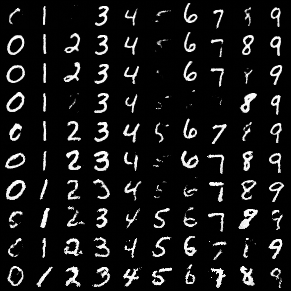
\includegraphics[width=.95\textwidth]{figures/MNIST/dif_temps.png}
    \\ (a)
\end{minipage}
\begin{minipage}{.1\textwidth}

\end{minipage}
\begin{minipage}[right]{.45\textwidth}
    \centering
    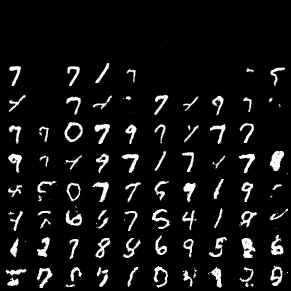
\includegraphics[width=.95\textwidth]{figures/MNIST/uncond_dif_temp_mnist.png}
    \\ (b)
\end{minipage}
\centering
\caption{(a): Class-conditional generated images from MNIST. The temperature of sampling increases from $0.1$ (top row) to $1.0$ (bottom row). Columns correspond to different classes. (b): Unconditional generated images from MNIST. The temperature of sampling goes from $0.1$ at top row to $1.0$ at bottom row. Columns are different random noise values.}
    \label{fig:cond_uncond_mnist}

\end{figure}

\end{document}
